
\documentclass[12pt,twocolumn,twoside]{article}
\usepackage{lingmacros}
\usepackage{tree-dvips}
\usepackage{graphicx}
\usepackage{caption}
\usepackage{subcaption}

\graphicspath{ {./img/} }

\begin{document}
	
	\title{Visual Analytics \\
		\large Engineering in Computer Science - Sapienza\\ Class 2019-2020}
	
	
	\author{Matteo Rizza, Nicola Di Santo}
	
	\twocolumn[
	\begin{@twocolumnfalse}
		\maketitle
		\begin{abstract}
			The main goal of this application is to allow users to visualize the interaction of the genes of available diseases. A set of filters and live analytics are provided that theoretically should allow users to better understand gene interaction and consequently formulate or validate hypotheses in the emerging field of network medicine. We are strongly inspired by the NEMESIS \cite{ivapp19} system but we adopted a slightly different approach by using a classic and widely used node-link diagram for displaying the interactome as well as a different kind of insights to the user. For the realization of the whole visual part, the \emph{d3.js}\cite{d3} library is used.
			
		\end{abstract}    
	\end{@twocolumnfalse}
	]
	
	
	\begin{center}
		\centering
		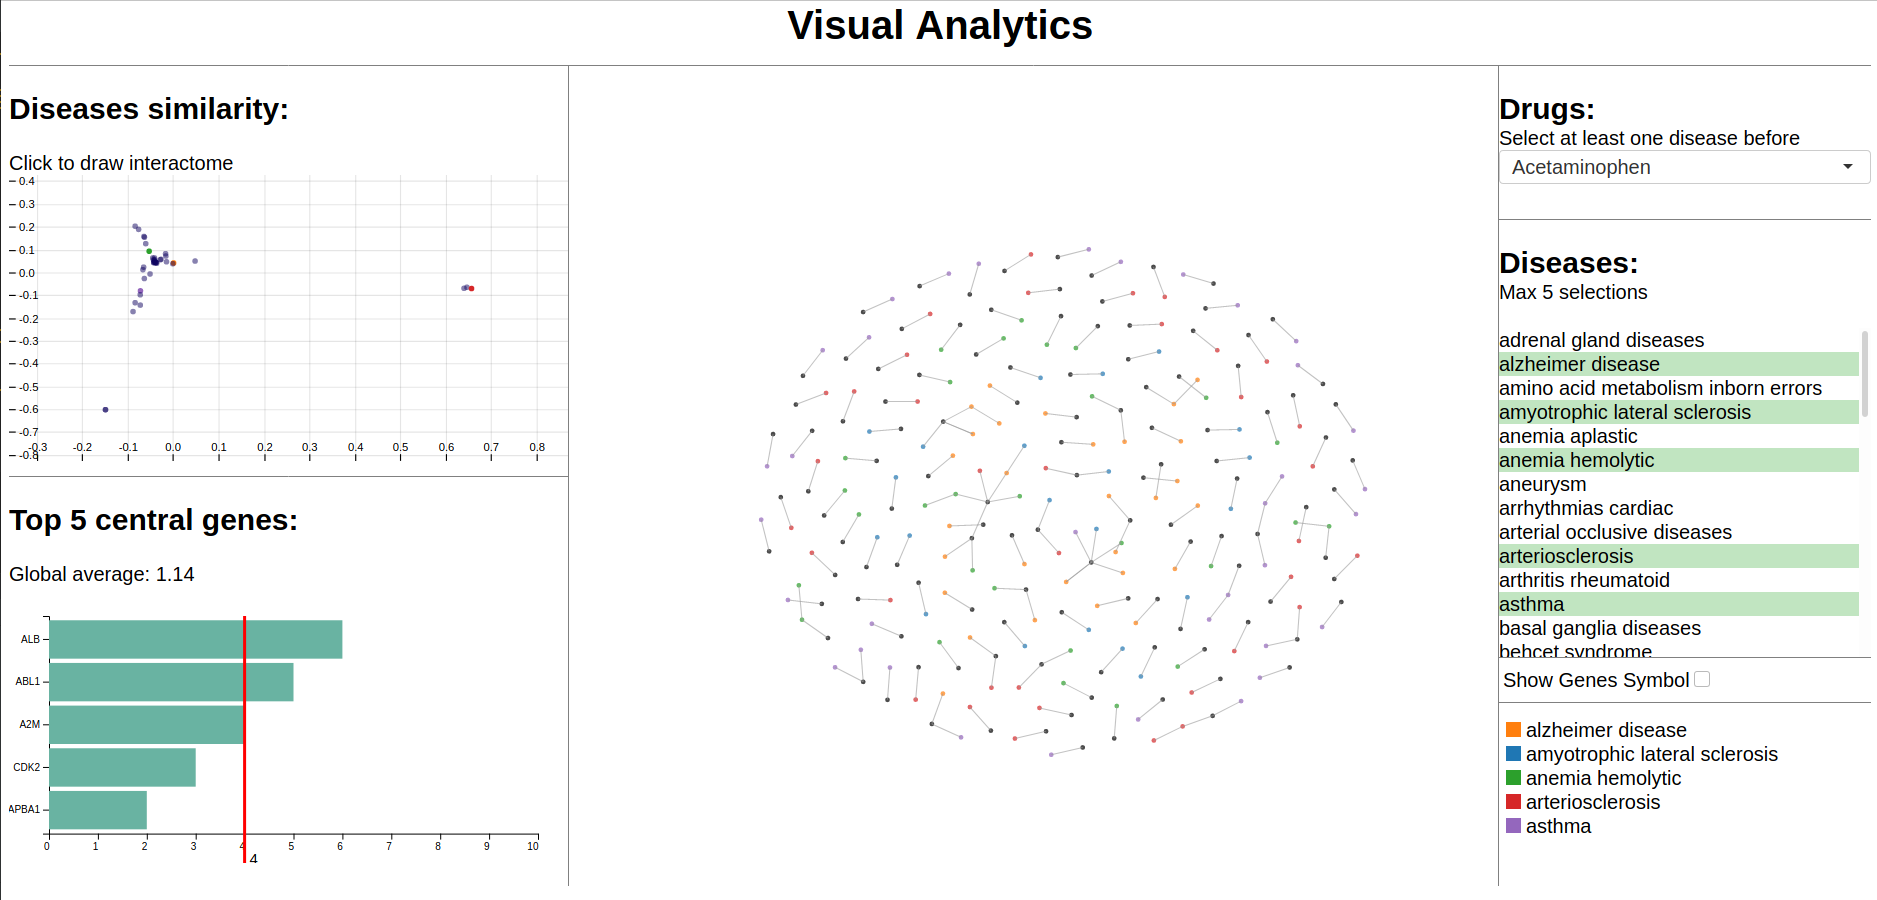
\includegraphics[height=70mm,width=.8\paperwidth,origin=center]{sys.png}
	\end{center}
	
	%Image of the system here
	
	\clearpage
	
	\section*{Introduction}
	The emerging tools of network medicine offer a platform to explore systematically not only the molecular complexity of a particular disease, leading to the identification of disease modules and pathways, but also the molecular relationships among apparently distinct phenotypes. Advances in this direction are essential for identifying new disease genes, for uncovering the biological significance of disease-associated mutations identified by genome-wide association studies and full-genome sequencing, and for identifying drug targets and biomarkers for complex diseases. This project tries to provide an interactive visual system to allow the operator to navigate and process this huge amount of graph-structured data to allow them to formulate a new hypothesis.\\ %talk about definitions
	In the following section, we will refer to the graph of interaction between genes as the interactome. Whenever we refer to ``the graph'' or ``the network'' without specifying what, we are using them as synonyms of interactome. 
	
	\section*{Dataset} %insert picture of data
	The datasets used in this project are from the OMIM (Online Mendelian Inheritance in Man) \cite{OMIM} project. It is a comprehensive, authoritative, and timely knowledge-base of human genes and genetic disorders compiled to support human genetics research and education and the practice of clinical genetics. \\
	From OMIM data we have used the Interactome Dataset, the Seeds Dataset and the Drug Target Dataset.\newline The Interactome Dataset is a relational dataset made of 141000. Each row is composed of five records, the first two represent a link between two genes expressed as id of source and target genes, the second two are the genes symbols (readable names) while the last one tells how this link was discovered. The Seeds dataset is a key-value dataset with as key the name of a disease and with value a list of genes involved in the relative disease. The last one is instead a mapping between drugs and genes it acts on. All those data have been exported from Excel format to TSV format and subsequently loaded into our application.\\ Since the interactome is very huge, to speed up the computations it is filtered and only links with source or target involved in at least one disease or drug are selected. This operation allows us to reduce its size of 70\% speeding up all the subsequent filtering necessary for visualization. The cut interactome dataset has $39000$ tuples, so even with this huge shrinking of interactome size and without considering the other datasets we still respect requirements of $AS_{index} > 10000$.
	
	\section*{The System}
	The system is composed of three main visualizations plus some filter components. When it is loaded for the first time only Diseases Scatterplot View and sidebar with filters are visible, all the other views depends on user selection.\\ 
	The user is allowed to select at most five diseases. To select a disease to analyze, he can use interchangeably either the scrollable sidebar on the right side of the screen or the scatterplot on the left upper corner of the screen. According to this selection, the interactome node-link diagram is displayed. Once the interactome network graph is visible the user is allowed to select a drug and understand if there is some gene of the interactome affected by that drug. Top 5 centrality genes are also computed for the interactome of selected diseases and they are displayed to the user in the left lower corner. All other view-specific interactions are explained in the next sections.
	\subsection*{Diseases Scatterplot View}
	The Disease Scatterplot View (Figure \ref{scatter}) is a scatterplot showing all the available disease to analyze. Each disease is represented as a point. To provide a better understanding of the scatterplot, by hovering a point with the mouse, a tooltip with the name of the corresponding disease is displayed. Each point has a $0.5$ opacity to make overlapping points visible. The view is zoomable so that very near points can be distinguished and further analyzed. The axes represent distances between points in a 2D reference frame and are scaled according to the zoom to make the user understand the degree of similarity between points. It is worth to point out that those are only relative distances between diseases and the coordinates themselves do not mean that much. \\ 
	To draw diseases as 2-D points we have, first of all, defined a distance measure between them. The distance is defined using Jaccard Similarity on the genes involved in the disease. Namely if we have two diseases $D_i$ and $D_j$ with $D_i$ acting on genes $G_i=\{g_{i1},g_{i2},...,g_{in}\}$ and $D_j$ acting on genes $G_j=\{g_{j1},g_{j2},...,g_{jm}\}$ where $G_j$ and $G_i$ are sets, we can compute the similarity between two disease as the Jaccard similarity on their set of genes: $J_s(D_i,D_j) = \frac{|G_i \cap G_j|}{|G_i \cup G_j|}$, the distance is simply $d =1-J_s(D_i,D_j)$.  Then the symmetric distance matrix between diseases is computed and multidimensional scaling (MDS) is applied on it to obtain 2-D points for each disease. We recall that an MDS algorithm places each object into N-dimensional space (N is an input parameter, $N=2$ in our case) such that the between-object distances are preserved as well as possible.\\ MDS is computed at the start-up of the system. We have used algorithm from \cite{mds_js}.
	
	\begin{figure}
		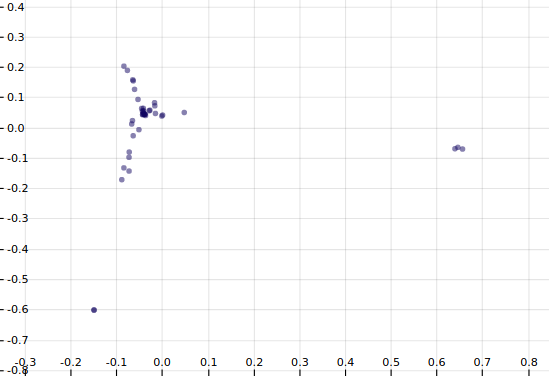
\includegraphics[width=.95\linewidth]{disease-scatterplot-mds.png}
		\caption{Disease scatterplot View}
		\label{scatter}
	\end{figure}
<<<<<<< HEAD
	This view is coordinated with the Diseases Interactome View and the sidebar disease selector in the sense that we can choose a disease to display in the interactome node-link diagram by either clicking on the sidebar selector or by clicking on a point in the scatterplot. Whenever we click on the sidebar selector entry, a point in the scatterplot corresponding to the selected disease is colored with the same color of the nodes of that disease in the Interactome View. Whenever we click on a scatterplot disease, the corresponding disease's nodes are drawn in the Interactome graph and the disease entry in the sidebar selector is focused in green.\\ The view can also be considered indirectly connected to the Top 5 Centrality View since it triggers an Interactome change that on its own side triggers changes on the Top 5 Centrality View. \\ 
	
	\subsection*{Diseases Interactome View}
	The Disease Interactome View (Figure \ref{net}) is a node-link diagram showing all the links between genes of the selected diseases. In this view, each gene is encoded as a node while each interaction between genes recorded in the interactome is encoded as a link. Each selected disease (up to five can be selected) has a color assigned to it, so basically we have encoded genes membership to a disease with colors.\\
	Inspired by NEMESIS\cite{ivapp19} work, we allow for degree one and degree two relationships. A degree two relationship is an indirect connection between two nodes with a path of length two. We obtain that connection by including not only links of the interactome with genes of the selected disease as extremes but also links containing only one gene of the selected disease as source or target.\newline All those interactions are encoded with a path of length equal to the degree of the path connecting the nodes. Some but not all relationships of degree greater than two can show up as side effects of the node-link representation, but they are not explicitly computed. To make clear to the users the nature of those interactions we have used a special encoding: each gene (node) affected by a disease is colored according to a color schema while each gene (node) connected with genes of that disease but not directly affected by the disease are colored of black.  This encoding allows to quickly recognize the nature of the relationship among genes of a disease.\\ 
	Each time a user adds one disease to the set of selected ones a color is assigned to it and a legend shows up.\\ The legend is clickable and clicks acts like selectors of diseases to focus on: if we select five diseases and then click on one of them in the legend, all the nodes lose their color and their opacity is reduced except for the selected ones. \\
	Whenever the Interactome View is not empty the user can also select a drug from the appropriate picker. If the selected drug acts on some displayed genes then its corresponding node size is increased with an animation to make the user aware of the relation.\\
	\begin{figure}
		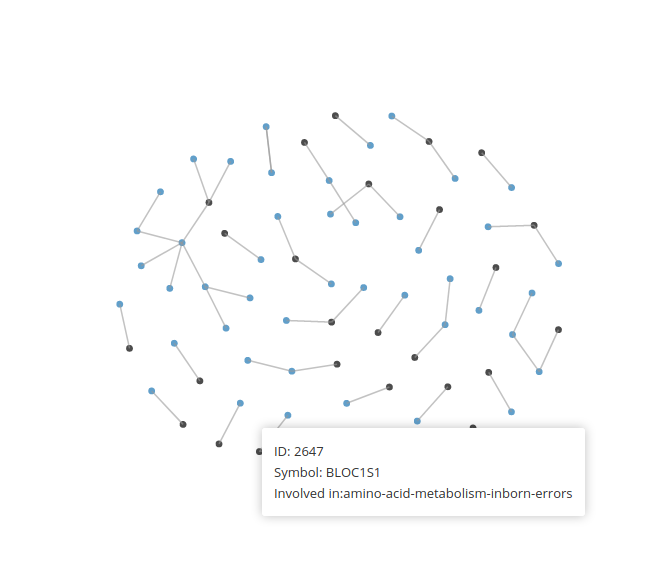
\includegraphics[width=.95\linewidth]{network.png}
		\caption{Disease Interactome View}
		\label{net}
	\end{figure}
	Nodes in the network also allows mouse hovering. Each time we hover the mouse on a node a tooltip shows up displaying gene's id, gene' symbol and disease it is involved in as visible in Figure \ref{net}.\\
	On the right corner of the network graph, it is possible to click on "Show Genes' Symbol" checkbox. This checkbox allows for displaying the name of each gene below its node. To fast distinguish those labels in dense graphs, the same color of the node(gene) is assigned to the respective label. It is important to note that this feature downgrades the user visualization experience of the interactome. We have decided to add it because we thought it might be useful for fast exploration. However, it is disabled by default and it is highly recommended to use it after selecting a disease in the legend as shown in Figure \ref{net2} to have the view as clean as possible.\\ 
	Since it is known that node-link diagrams some times are difficult to read due to limited space and the huge amount of graphics element (especially if genes symbols are also displayed), we have added the last chance possibility to drag nodes around to place them was the user prefer from a readability point of view, but we hope this feature is never needed.
	
	\begin{figure}
		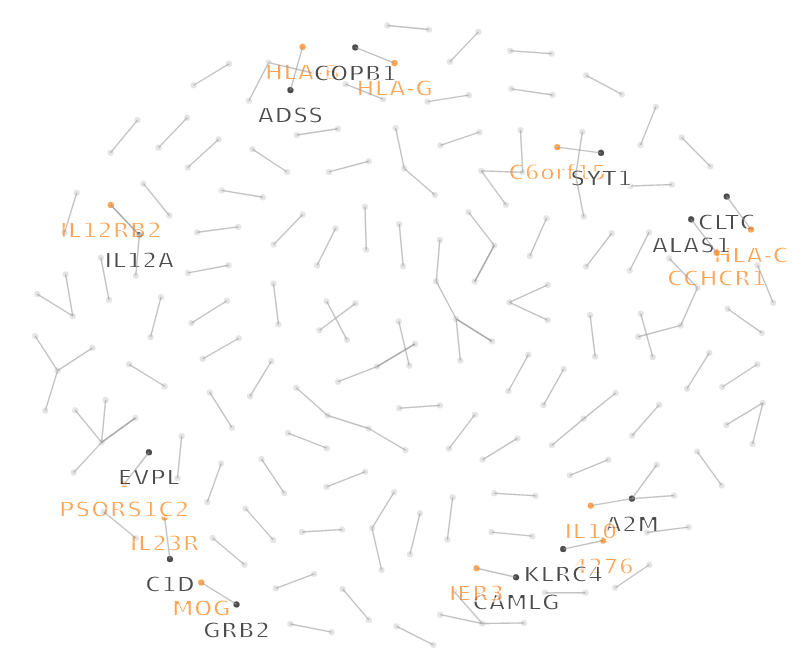
\includegraphics[width=.95\linewidth]{net2.png}
		\caption{Gene Symbol View Explicit}
		\label{net2}
	\end{figure}
	
	
	\subsection*{Top 5 Centrality View}
	The Top 5 Centrality View (Figure \ref{top5}) computes and shows Centrality statistics for the displayed interactome. In graph theory and network analysis, indicators of centrality identify the most important vertices within a graph.  In this work, we have tried to define centrality as the number of connections a gene has, hence recalling the definition of centrality for social graphs. It is computed live and only for the displayed genes, hence a node that has a great centrality in the full interactome, here can have a low centrality, meaning that it has low influence within the selected diseases. \\ The top 5 is displayed as a horizontal bar-chart where the width of a bar encodes the centrality measure. The vertical axes labels indicate gene symbol while the horizontal axes quantifies centrality.\newline Two types of centrality means are also displayed: the first one, encoded as a vertical red line on the bar chart, represent the top 5 centrality mean; the second one, encoded as simple text, represent the overall centrality mean of the displayed interactome. With those two measures, the user can understand if high centrality is a characteristic of the whole selected interactome or only of a restricted subset of genes. Namely in figure \ref{top5} we can see mean centrality of the top 5 has value 4.8 while global average of the displayed network is 1.23, that makes us understand that nodes with high centrality in the selected interactome are exceptions.\\ By hovering with mouse on the bars the user can see the relative gene in the interactome since an animation is triggered increasing the node radius.
	
	\begin{figure}
		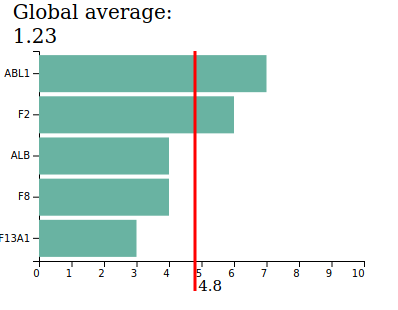
\includegraphics[width=.95\linewidth]{top5.png}
		\caption{Top 5 Centrality Genes}
		\label{top5}
	\end{figure}
	
	\subsection*{Coordination Between Views}
	In this paragraph, we briefly summarize the coordination between views.\newline The scatterplot view is directly coordinated with the Interactome View and with the side disease selector, indirectly with the top 5 view, since triggering a selection will automatically change the displayed interactome and hence the top 5 centrality view.
	The top 5 centrality view is connected directly with the interactome graph since it allows to focus top 5 genes in the network as explained above. the network itself does not trigger changes on other components but it is affected by all of them. The legend acts on the network as explained above and it shares the same color schema with the interactome nodes and with the scatterplot points (recall colors represent diseases). The disease selector is coordinated together with the network and the scatterplot, the drug selector affects only the network.
	
	
	\subsection*{Analytics Summary}
	Here we briefly summarize analytics of the system.\newline The dataset, mainly composed of interactome data is filtered each time the system is loaded. The time required to load and process those data is printed in the console and is about 300 milliseconds on an Intel-i5-7thGen machine. Immediately after (Javascript is single-threaded), we compute MDS on loaded data as explained in the scatterplot view section using plain Javascript code. Each time we select some diseases to be displayed the graph is built on the fly, isolating from the interactome network only values of interest. Each time a new network is available, the top 5 centrality computation and global centrality computation are triggered.
	
	\subsection*{Conclusions}
	With this visualization system, heavily inspired by NEMESIS \cite{ivapp19}, we have tried to provide a complementary view for less expert users with the well-know node-link diagram. Accordingly to it, we also visualize degree one and two relationships between genes. Differently from NEMESIS, we gave freedom to the users to drive their research into a disease-based manner by making available a complete list of diseases and giving the possibility of select the diseases of interest. In conclusion, our system aspires to become an integration rather than an alternative to NEMESIS to provide a 360-degree view to the potential users and satisfy their needs.
	\clearpage
	\bibliographystyle{unsrt}
	\bibliography{citazioni} 
	
=======
This view is coordinated with the Diseases Interactome View and the sidebar disease selector in the sense that we can choose a disease to display in the interactome node-link diagram by either clicking on the side bar selector or by clicking on a point in the scatterplot. Whenever we click on the sidebar selector entry, a point in the scatterplot corresponding to the selected disease is colored with the same color of the nodes of that disease in the Interactome View. Whenever we click on a scatterplot disease, the corresponding disease's nodes are drawn in the Interactome graph and the disease entry in the sidebar selector is focused in green.\\ The view can also be considered indirectly connected to the Top 5 Centrality View, since it triggers an Interactome change that on its own side triggers changes on the Top 5 Centrality View. \\ 

\subsection*{Diseases Interactome View}
The Disease Interactome View (Figure \ref{net}) is a node-link diagram showing all the link between genes of the selected diseases. In this view each gene is encoded as a node while each interaction between genes recorded in the interactome is encoded as a link. Each selected disease (up to five can be selected) has a color assigned to it, so basically we have encoded genes disease relation with colors.\\
Inspired by NEMESIS\cite{ivapp19} work, we allow for degree one and degree two relationships. A degree two relationship is basically a indirect connection between two nodes with a path of length two. We obtain those connection by including not only links of the interactome with genes of the selected disease as extremes but also links containing only one gene of the selected disease as source or target.\newline All those interaction are encoded with path of length equal to the degree of the path connecting the nodes. Some but not all relationship of degree greater than two can show up as side effect of the node-link representation, but they are not explicitly computed. To make clear to the users the nature of those interaction we have used a special encoding: each gene (node) affected by a disease is colored according to a scale while each gene (node) connected with genes of that disease but not directly affected by the disease are colored of black.  This encoding allows to quickly recognize the nature of relationship among genes of a disease.\\ 
Each time a user add one disease to the set of selected ones a color is assigned to it and a legend shows up.\\ The legend is clickable and clicks acts like selector of diseases to focus on: if we select five diseases and then click on one of them in the legend, all the nodes loose their color and their opacity is reduced except for the selected ones. \\
Whenever the Interactome View is not empty the user can also select a drug from the appropriate picker. If the selected drug acts on some displayed genes then its corresponding node size is increased with an animation to make the user aware of the relation.\\


\begin{figure}
	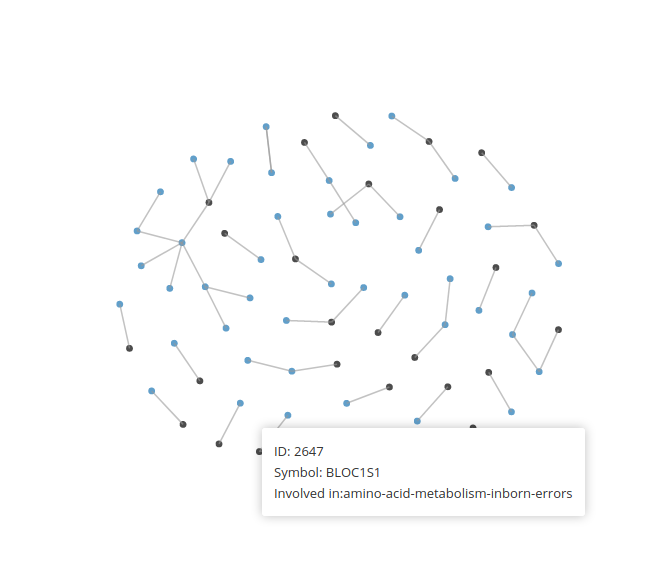
\includegraphics[width=.95\linewidth]{network.png}
	\caption{Disease Interactome View}
	\label{net}
\end{figure}

Nodes in the network also allows mouse hovering. Each time we hover the mouse on a node a tooltip shows up displaying gene's id, gene' symbol and disease it is involved in as visible in Figure \ref{net}.\\
On the right corner of the network graph it is possible  click on "Show Genes' Symbol" checkbox. This checkbox allows for displaying the name of each gene below its node. To fast distinguish those labels in dense graphs, the same color of the node(gene) is assigned to the respective label. It is important to note that this feature actually downgrades the user visualization experience of the interactome. We have decided to add it because we thought it might be useful for fast exploration or a user. However it is disabled by default and it is a full responsibility of the user to use it properly. It is highly recommended to use it after selecting a disease in the legend as shown in Figure \ref{net2} to have the view as clean as possible.\\ 
Since it is known that node-link diagrams some times are difficult to read due to limited space and huge amount of graphics element (especially if genes symbols are also displayed), we have added the last chance possibility to drag nodes around to place them were the user prefer from a readability point of view, but we hope this feature is never needed.

\begin{figure}
	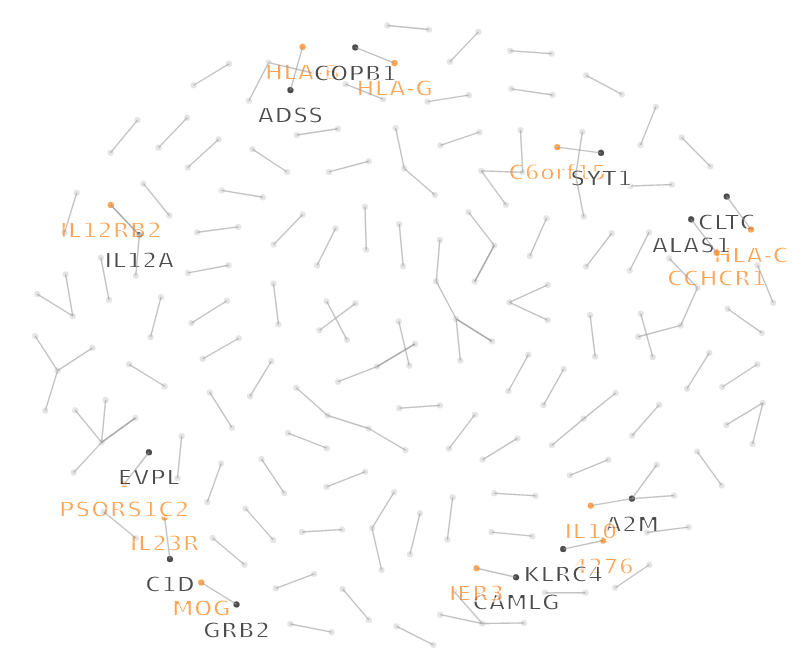
\includegraphics[width=.95\linewidth]{net2.png}
	\caption{Gene Symbol View Explicit}
	\label{net2}
\end{figure}


\subsection*{Top 5 Centrality View}
The Top 5 Centrality View (Figure \ref{top5}) computes and show Centrality statistics for the displayed interactome. In graph theory and network analysis, indicators of centrality identify the most important vertices within a graph.  In this work we have tried to give a definition of centrality as the number of connection a gene has, hence recalling the definition of centrality for social graphs. It is computed live and only for the displayed genes, hence a node that has a great centrality in the full interactome, here can have a low centrality, meaning that it has low influence within the selected diseases. \\ The top 5 is displayed as a horizontal bar-chart where the width of a bar encodes the centrality measure. The vertical axes labels gene symbol while the horizontal axes quantifies centrality.\newline Two types of centrality means are also displayed: the first one, encoded as a vertical red line on the bar chart, represent the top 5 centrality mean; the second one, encoded as simple text, represent the overall centrality mean of the displayed interactome. With those two measures the user can understand if high centrality is a characteristic of the whole selected interactome or only of a restricted subset of genes. Namely in figure \ref{top5} we can see mean centrality of the top 5 has value 4.8 while global average of the displayed network is 1.23, that makes us understand that nodes with high centrality in the selected interactome are exceptions.\\ By hovering with mouse on the bars the user can see the relative gene in the interactome since an animation is triggered increasing the node radius.

\begin{figure}
	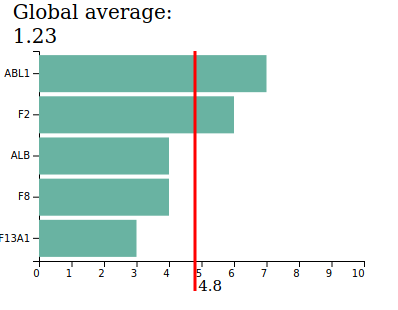
\includegraphics[width=.95\linewidth]{top5.png}
	\caption{Top 5 Centrality Genes}
	\label{top5}
\end{figure}

\subsection*{Coordination Between Views}


\subsection*{Analytics Summary}

\clearpage
\bibliographystyle{unsrt}
\bibliography{citazioni} 

>>>>>>> parent of e44337e... borderfix
\end{document}